\subsection{Digital front end}\label{sec:frontend}
The digital front end consist of two parts, D flip flop and NAND/NOR gate.  The D flip flop will synchronise the incoming date and the NAND/NOR gate will modulate the signal with the local oscillator.This signal will go to the level shifter. The two parts will be described in this paragraph.

\subsubsection{D flip flop}\label{sec:frontend}
A D flip flop will be used to synchronise the incoming thermometer coded data and to ensure that the output pmos and nmos switch at the same time. There are a couple of challenges that are important to take into account when designing a D flip flop, for example the operation speed and the transition time of the output at the rising clock. 
A flip flop can be made in different ways. The two main technologies are in CMOS and CML. The CMOS design is relative less complex in compare to CML, but in CML there are more parameters that can be modified to tune the output. In this project the CMOS design is used, because it is less complexity, single-ended and it can be realised in a short time period.  The CMOS circuit of previous group is used in this project, ~\cite{coursebook} - ~\cite{powerdac}, but the size of the pmos is changed to get a better performance. The schematic is shown in Fig.~\ref{fig:D_flip_flop_schematic}. The D flip flop works with a master-slave principal. The master will set the data on the rising clock and it keeps it until the clock is low. The slave will copy the data of the master and hold the data when the clock is low. 

To explain this principal in the schematic, the diagram can be divided into three parts, settle time of the data, master latch and slave latch. In the first part the data will be set when the clock is low. The second part, the master latch will set the settled data and when the clock is high it will set the data to the output of the master latch and the first part will be turned off. The third part, the slave latch will follow the master latch when the clock is high, but when the clock is low the master latch output will be turned off and slave latch will be holding the data. 
\begin{figure}[h]
 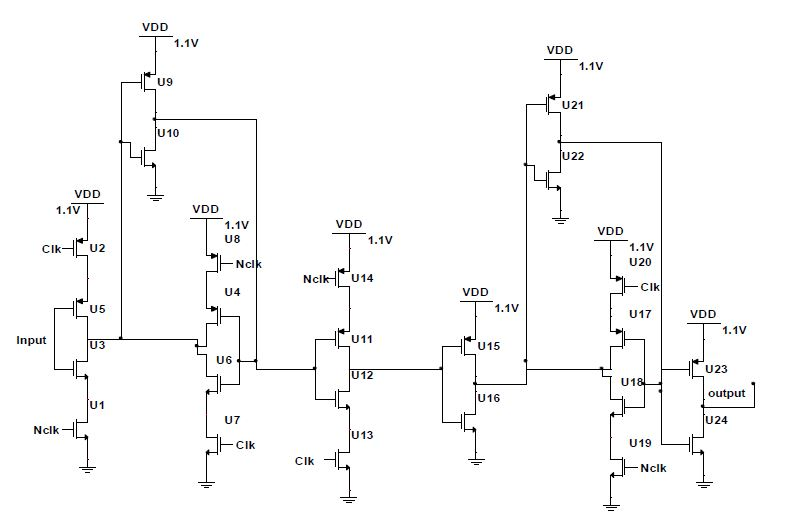
\includegraphics[width=0.5\textwidth]{D_flip_flop_schematic}
 \caption{D flip flop schematic, this schematic will be updated in the next version to define the parts better.}
 \label{fig:D_flip_flop_schematic}
\end{figure}
The size of all of the nmos are 50nx90n(length x width). The width of the pmos is determined with the simulation to get smallest delay between the rising clock and the output. The pmos have the following dimensions: 50nx180nm (length x width). The bulk of the pmos is connected to the power supply (1.1V) and the bulk of the nmos is connected to the ground.

The rise time, fall time, critical point graph will be shown in the next version. 

\subsubsection{NAND/NOR gate}\label{sec:frontend}
The NAND and NOR will modulate the local oscillator signal (LO) with the data from the D flip flop. The LO signal works with a 2Ghz square wave. 
The design of the NAND and NOR will be in the next version of the paper.


